\documentclass[12pt]{kiarticle}
\graphicspath{{pictures/}}
\DeclareGraphicsExtensions{.pdf,.png,.jpg,.eps}
%%%
\pagestyle{fancy}
\fancyhf{}
%\renewcommand{\headrulewidth}{ 0.1mm }
\renewcommand{\footrulewidth}{ .0em }
\fancyfoot[C]{\texttt{\textemdash~\thepage~\textemdash}}
\fancyhead[L]{Вопрос по выбору --- оптика, 2018\hfil}
\fancyhead[R]{\hfil Иванов Кирилл, 625 группа }
\usepackage{multirow} % Слияние строк в таблице
\newcommand
{\un}[1]
{\ensuremath{\text{#1}}}
\newcommand{\eds}{\ensuremath{ \mathscr{E}}}
\usepackage{tikz}
%%% Работа с таблицами
\usepackage{array,tabularx,tabulary,booktabs} % Дополнительная работа с таблицами
\usepackage{longtable}  % Длинные таблицы
\usepackage{multirow} % Слияние строк в таблице

\begin{document}
	
	\begin{titlepage}
	\begin{center}
		\large 	Московский физико-технический институт \\
		(государственный университет) \\
		Факультет общей и прикладной физики \\
		\vspace{0.2cm}
		
		\vspace{4.5cm}
		\Large{Вопрос по выбору в 4 семестре \\ \vspace{0.2cm}
			(Общая физика: оптика)} \\ \vspace{0.2cm}
		\LARGE \textbf{Модовый состав лазерного излучения}
	\end{center}
	\vspace{2.3cm} \large
	
	\begin{center}
		Работу выполнил: \\
		Иванов Кирилл,
		625 группа
		\vspace{10mm}		
		
	\end{center}
	
	\begin{center} \vspace{60mm}
		г. Долгопрудный \\
		2018 год
	\end{center}
\end{titlepage}



\section{Введение}

\textbf{Лазер} ---  источник квазимонохроматического и узконаправленного высококогерентного потока излучения, работающий за счёт квантово-механического эффекта вынужденного (индуцированного) излучения.

Главными элементами лазера являются \textbf{оптический резонатор} и расположенная в нём \textbf{активная среда}, способная усиливать проходящее через неё излучение.

\begin{figure}[h!]
	\centering
	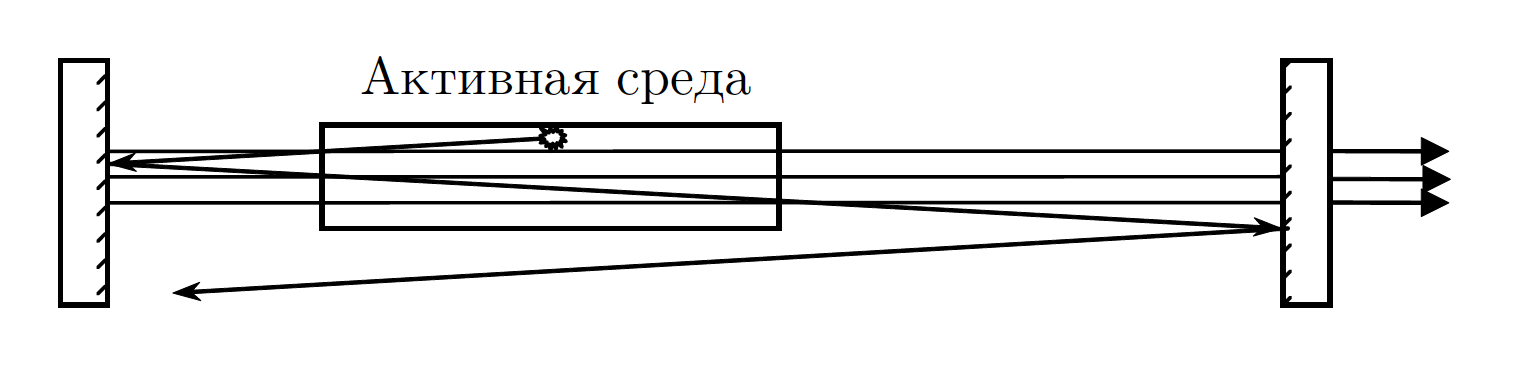
\includegraphics[width=0.7\linewidth]{laser.png}
	\caption{Схема лазера}
	\label{laser}
\end{figure}

\subsection{Квантово-механическое введение}

В силу выхода квантовой физики и связанных с ней явлений за рамки нашего курса мы не будем подробно останавливаться на квантово-механических принципах работы лазера.

Если вкратце, то из-за \textbf{спонтанного} (самопроизвольного) излучения электронами фотонов с энергией $ E = \hbar \omega $ появившиеся частицы света возбуждают атомы, заставляя их переходить на следующий энергетический уровень $ E_1 = E_0 + \hbar \omega $. После взаимодействия других фотонов с уже возбужденными электронами происходит \textbf{вынужденное} излучение, после чего атом возвращается в основное состояние. В результате этих процессов возникает электромагнитная волна с частотой $ \omega = \dfrac{E_1 - E_0}{\hbar} $, которая усиливается за счёт взаимодействия с активной средой.  

Конечно, нужно понимать, что в реальности такие волны являются не монохроматическими с бесконечно узкой линией поглощения/излучения $ \omega $, а обладают конечной шириной $ \Delta \omega $, которая называемся шириной спектра усиления активной среды лазера (\textbf{спектра генерации}). Она определяется из квантовых и иных характеристик атомов и активной среды. 

\subsection{Роль резонатора}

Простейший резонатор представляет собой \textbf{интерферометр
Фабри–Перо}, состоящий из двух плоских зеркал с
высокими коэффициентами отражения, размещённых параллельно друг другу на фиксированном расстоянии. Благодаря наличию
активной среды, в резонаторе многократно усиливаются волны, распространяющиеся вдоль оси системы и набирающие за один полный
проход резонатора фазу, кратную $ 2\pi $ (т.е. на оптической длине резонатора укладывается целое число полуволн, в системе при этом
образуются \textbf{стоячие волны}). Таким образом, резонатор обеспечивает
создание положительной обратной связи в лазере и превращает его
в генератор излучения. Также в резонаторе происходит накопление
энергии излучения и отбор узких резонансных линий из спектра
излучения, рождающегося в среде. Одно из зеркал резонатора обычно
имеет несколько меньший коэффициент отражения, что позволяет
выпускать через него часть излучения в виде узконаправленного
высокомонохроматического пучка.

\section{Модовый состав лазерного излучения}

\textbf{Модами} называют стационарные типы колебаний электромагнитного поля в резонаторе, различающиеся частотой и пространственным распределением амплитуды поля.

Рассмотрим моды в открытом резонаторе Фабри–Перо с плоскими
зеркалами, расстояние между которыми равно $ L $. Будем считать, для
простоты, что активная среда заполняет весь резонатор и имеет показатель преломления $ n= 1 $.

\newpage
\section{Экспериментальный подсчет числа мод}

\newpage
\section{Селекция продольных мод}


\newpage
\section{Заключение}

\section*{Использованная литература}

\begin{itemize}
	
	\item Звелто "<Принципы лазеров
	
	\item Лабник
	
\end{itemize}



\end{document}